\documentclass[11pt]{article}

\usepackage[utf8]{inputenc}
\usepackage[margin=0.8in]{geometry}
\usepackage{graphicx}
\graphicspath{{img/}}
\usepackage{float}
\usepackage{amsmath}
\usepackage{amssymb}
\usepackage{setspace}
\usepackage{enumitem}
\usepackage{titlesec}
\usepackage[version=4]{mhchem}
\usepackage{siunitx}
\usepackage{multicol}
\usepackage{caption}
\usepackage{gensymb}

\newenvironment{tight_enumerate}{
\begin{enumerate}[label=(\alph*)]
\setlength{\itemsep}{3pt}
\setlength{\parskip}{0pt}
}{\end{enumerate}}

\titleformat*{\section}{\large\bfseries}
\titleformat*{\subsection}{\normalsize\bfseries}

\title{\vspace{-2em} \textbf{Homework 2}}
\author{Justin Kang \\ AST 381: Star Formation}
\date{\vspace{-0.75em} October 3, 2018}

\begin{document}
\maketitle
\singlespacing
\pagenumbering{gobble}
\sloppy


\vspace{-2em}
\section*{Problem 1. Spherical Cows, I mean, Clouds}
\begin{tight_enumerate}
\item Consider a spherical isothermal cloud at zero temperature with a constant density $\rho_{0}$. There is no magnetic field. If the cloud is at rest at $t = 0$, show that it will collapse to a point at a time 
\[t_{\text{ff}} = \left(\frac{3\pi}{32G\rho_{0}}\right)^{1/2}.\]
\item Using the virial theorem, show that the maximum mass of an isothermal sphere of constant density is
\[M_{\text{max}} = 1.77\frac{c_{0}^{4}}{\sqrt{G^{3}p_{0}}},\]
where $c_{0}$ is the isothermal sound speed and $p_{0}$ is the ambient pressure. If the unphysical assumption of constant density is dropped, one finds that the maximum stable mass has the same form as above, but with a coefficient of 1.18; $M_{\text{max}}$ is now the Bonnor-Ebert mass.
\item Define the virial parameter as 
\[\alpha \equiv \frac{5\sigma^{2}R}{GM},\]
where $\sigma$ is the 1D velocity dispersion. This is convenient because each of the parameters can be estimated from observations. Let $v_{A} = \bar{B}/(4\pi\bar{\rho})^{1/2}$ be the Alfv\'en velocity in terms of the mean field and mean density of the cloud. Assuming the cloud is spherical, show that the Alfv\'en Mach number can be written
\[M_{A} \equiv \frac{\sigma}{v_{A}/\sqrt{3}} \equiv \frac{\sqrt{\alpha}}{1.98}\left(\frac{M}{M_{\Phi}}\right),\]
where $M_{\Phi} \equiv 0.12\Phi/\sqrt{G}$ is the magnetic critical mass. This identity shows that if the virial parameter is of order unity then $M_{A}$ is as well, provided the cloud is slightly magnetically supercritical: $M \simeq 2M_{\Phi}$.
\end{tight_enumerate}

\subsection*{Solution 1}
\begin{tight_enumerate}
\item Suppose there is a particle at radius $R$ from the cloud, which has a uniformly distributed mass $M$. Gravitational collapse can be considered as half of a Keplerian orbit with $a = R/2$ and $e = 1$. The free fall time is then given by $t_{\text{ffc}} = P/2$, where $P$ is the period of the orbit. Using Kepler's third law, this then becomes 
\[t_{\text{ff}} = \frac{1}{2}\left[\frac{4\pi^{2}}{GM}\left(\frac{R}{2}\right)^{3}\right]^{1/2} = \left(\frac{\pi^{2}R^{3}}{8GM}\right)^{1/2} = \left(\frac{3\pi}{32G}\frac{\frac{4}{3}{\pi}R^{3}}{M}\right)^{1/2} = \left(\frac{3\pi}{32G\rho_{0}}\right)^{1/2}.\]
\fbox{$\therefore$ $t_{\text{ff}} = \left(\frac{3\pi}{32G\rho_{0}}\right)^{1/2}$}
\newpage
\item In this case, we know that there is a balance between kinetic and gravitational energy. The virial theorem can then be written as 
\[\frac{1}{2}\frac{d^{2}I}{dt^{2}} = 2(T-T_{S}) + W,\]
where $I$ is the moment of inertia, $T$ is the total kinetic energy, $T_{S}$ the confining pressure at the cloud surface, and $W$ the gravitational energy. Expanding each of these terms out, we can write
\[T = \int_{V}{\left(\frac{1}{2}{\rho}v^{2}+\frac{3}{2}P\right)dV} = \frac{1}{2}\left(\frac{4}{3}{\pi}R^{3}\right){\rho}v^{2} + \frac{3}{2}PV = \frac{1}{2}Mv^{2} + 2{\pi}R^{3}p_{0},\]
\[T_{S} = \int_{S}{\mathbf{r} \cdot ({\rho}v^{2} + P\mathbb{I}) \cdot dS} = 4{\pi}R^{3}p_{0},\]
\[W = -\frac{3}{5}\frac{GM^{2}}{R}.\]
Here we have neglected the ram pressure. For a cloud in equilibrium $\frac{d^{2}I}{dt^{2}} = 0$. Setting $v$ as the root mean square velocity, $v^{2} = 3\left(\frac{k_{b}T}{m}\right) = 3c_{0}^{2}$. The virial theorem can then be written as 
\[4{\pi}R^{3}p_{0} = 3Mc_{0}^{2} - \frac{3}{5}\frac{GM^{2}}{R}.\]
Solving for the mass, we find that 
\[M = \frac{R}{6G}\left(\sqrt{225c_{0}^{4}-240{\pi}R^{2}Gp_{0}}+15c_{0}^{2}\right).\]
We want to find where $M$ is maximized, so we take the derivative with respect to $R$ and set it equal to 0. This gives us the value of $R$:
\[R = \frac{3\sqrt{5}}{8\pi}\frac{c_{0}^{2}}{\sqrt{Gp_{0}}}.\]
Plugging this back into our expression for $M$, we find that 
\[M = \frac{45\sqrt{5}}{32\sqrt{\pi}}\frac{c_{0}^{4}}{\sqrt{G^{3}p_{0}}} \approx 1.77\frac{c_{0}^{4}}{\sqrt{G^{3}p_{0}}}\]
\fbox{$\therefore$ $M_{\text{max}} = 1.77\frac{c_{0}^{4}}{\sqrt{G^{3}p_{0}}}$}
\newpage
\item Given that the 1D velocity dispersion is $\sigma$, the 3D velocity dispersion is given by $\sqrt{3}\sigma$. The Alfv\'en Mach number is defined as $M_{A} = \frac{v}{v_{A}}$. By making the approximation that the velocity in the cloud is equivalent to the 3D dispersion, we find that $M_{A} = \frac{\sqrt{3}\sigma}{v_{A}} = \frac{\sigma}{v_{A}/\sqrt{3}}$.\\
\fbox{$\therefore$ $M_{A} \equiv \frac{\sigma}{v_{A}/\sqrt{3}}$}\\
Rearranging our definition of the virial parameter, we find that the 1D velocity dispersion can be written as 
\[\sigma = \left(\frac{GM\alpha}{5R}\right)^{1/2}.\]
The mean magnetic field is derived from the potential following the equation 
\[\Phi = \int{B \cdot dA} = {\pi}R^{2}B,\]
so substituting this in for the Alfv\'en velocity and plugging all of this into our expression for $M_{A}$, we find that 
\[M_{A} = \frac{\sigma}{v_{A}/\sqrt{3}} = \frac{\sqrt{3}\left(\frac{GM\alpha}{5R}\right)^{1/2}}{\left(\frac{\Phi}{{\pi}R^{2}\sqrt{4\pi\bar\rho}}\right)} = \frac{\sqrt{3}(GM\alpha)^{1/2}{\pi}R^{2}\sqrt{4\pi\bar\rho}}{(5R)^{1/2}\Phi}.\]
Making the substitution $\bar\rho = \frac{M}{\frac{4}{3}{\pi}R^{3}}$, 
\[M_{A} = \frac{\sqrt{3}(GM\alpha)^{1/2}{\pi}R^{2}\sqrt{4{\pi}M/\left(\frac{4}{3}{\pi}R^{3}\right)}}{(5R)^{1/2}\Phi} = \frac{3\pi}{\sqrt{5}}\sqrt{\alpha}\left(\frac{M}{\Phi/\sqrt{G}}\right)\]
We find that $\frac{3\pi}{\sqrt{5}} \approx \left(\frac{1}{1.98}\right)\left(\frac{1}{0.12}\right)$, thus
\[M_{A} = \frac{\sqrt{\alpha}}{1.98}\left(\frac{M}{0.12\Phi/\sqrt{G}}\right) = \frac{\sqrt{\alpha}}{1.98}\left(\frac{M}{M_{\Phi}}\right).\]
\fbox{$\therefore$ $M_{A} \equiv \frac{\sqrt{\alpha}}{1.98}\left(\frac{M}{M_{\Phi}}\right)$}
\end{tight_enumerate}


\newpage
\section*{Problem 2. Observing Real, Star-Forming Cows}
This problem uses real observations of different CO isotopologues of a nearby molecular cloud. I have uploaded \ce{^{12}CO} (1-0), \ce{^{13}CO} (1-0), and \ce{C^{18}O} (1-0) maps of the protostellar cluster NGC1333 in the Perseus molecular cloud complex, obtained using the $14$-m radio telescope at the Five College Radio Observatory (FCRAO), which used to be in MA. The \ce{^{12}CO} map was obtained as part of the COMPLETE survey of Perseus (Ridge et al. 2006, ApJ, 131, 2921). The \ce{^{13}CO} and \ce{C^{18}O} maps were obtained simultaneously and are part of a survey of the molecular gas surrounding a sample of protostellar clusters (Ridge et al. 2003, ApJ, 126, 286).\\
\indent First download these fits cubes from Canvas: ngc1333\_12co.fits, ngc1333\_13co.fits, and ngc1333\_c18o.fits. Note the first cube is the "mystery" data cube from problem set 1.\\
\indent Before starting this problem I suggest reading $\S15.4$ in Chapter $15$ of "Tools of Radio Astronomy" (by Tom Wilson et al.). This book is available in the Astronomy-Physics-Math library. For this problem you should assume the following:
\begin{itemize}
\item The efficiency of the FCRAO telescope is such that $T_{A} = 0.5\ T_{B}$
\item The distance to NGC1333 is $280\ \si{pc}$ (Zucker, C. et al. 2018 arXiv)
\item The velocity axis shows the velocity with respect to the Local Standard of Rest ($v_{\text{LSR}}$) and goes from $-9.995$ to $29.995$ \si{km/s}, with channel widths of $0.133\ \si{km/s}$.
\item Pixels are $25" \times 25"$
\end{itemize}
\begin{tight_enumerate}
\item Make integrated intensity maps from the different line maps for the velocity range $3.5 < v_{\text{LSR}} < 12.0\ \si{km/s}$. Describe the maps in words and discuss their similarities and differences.
\item Obtain an excitation temperature map of the cloud using the peak emission of the \ce{^{12}CO} in each pixel. Discuss how you produced the map, your calculations, and findings.
\item Calculate the mass of the cloud for the same velocity range as above, using each of the three maps and assuming all lines are optically thin. Discuss your results. Compare your mass estimate using the \ce{^{12}CO} with the other two estimates. Why are they different or the same?
\item Now obtain the mass using the \ce{^{13}CO} (1-0) map, taking into consideration the line optical depth, and compare any differences or similarities with the mass estimate obtained from the \ce{C^{18}O} (1-0) map (above). Note that in the literature there are various ways to correct for opacities. Choose one technique and explain the assumptions and the method thoroughly.
\item Use your mass estimates and the velocity dispersion derived in HW 1 to compute the virial parameter under the optically thick and thin assumptions. Discuss the results.
\end{tight_enumerate}
The following papers may also be helpful:\\
Appendix of Bourke et al. 1997, ApJ, 476, 781\\
Appendix of Pineda et al. 2011, ApJ, 743, 201\\
Body and appendix of Dunham et al. 2014, 783, 29\\
Appendix of Zhang et al. 2016, ApJ, 832, 158

\newpage
\subsection*{Solution 2}
\begin{tight_enumerate}
\item \leavevmode
\begin{multicols}{2}
\begin{figure}[H]
\centering
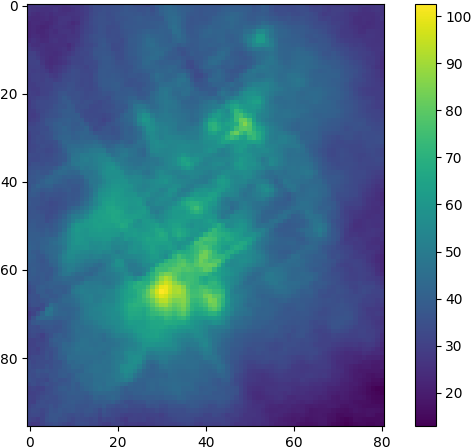
\includegraphics[width=0.4\textwidth]{12co_intensity.png}
\caption*{The integrated intensity map for \ce{^{12}CO}.}
\end{figure}
\begin{figure}[H]
\centering
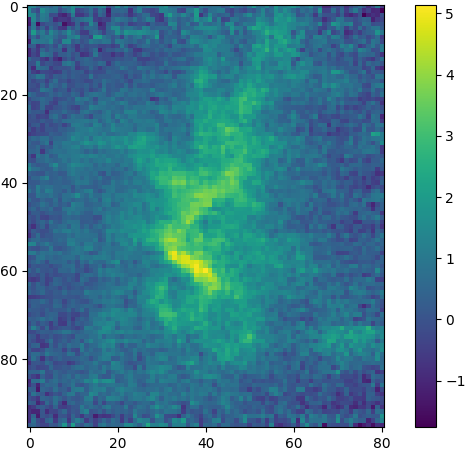
\includegraphics[width=0.4\textwidth]{c18o_intensity.png}
\caption*{The integrated intensity map for \ce{C^{18}O}.}
\end{figure}
\begin{figure}[H]
\centering
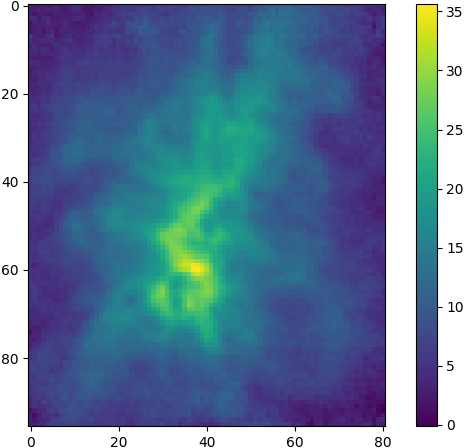
\includegraphics[width=0.4\textwidth]{13co_intensity.png}
\caption*{The integrated intensity map for \ce{^{13}CO}.}
\end{figure}
\begin{figure}[H]
\centering
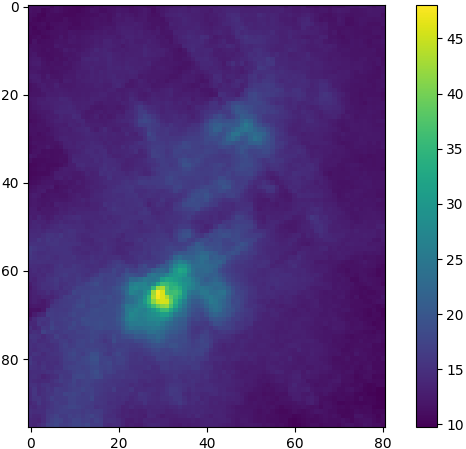
\includegraphics[width=0.4\textwidth]{temp.png}
\caption*{The excitation temperature map.}
\end{figure}
\end{multicols}
The integrated intensity maps have all brighter regions in the lower left quadrant, which is indicative of concentrations of gas. From Homework 1, we expect this region to be star forming, which would be these concentrated regions. All three of these maps also relatively share the same brightness structure. We find that the \ce{^{12}CO} map has the highest overall intensity and a lot more detail, and indicates possibly two regions of concentrated gases. As we go to the isotopologues, we find that the intensity reduces by an order of magnitude, and features tend to become blurrier and less defined. This can be attributed to the fact that \ce{^{13}CO} is less abundant than \ce{^{12}CO}, and \ce{C^{18}O} even less so. 
\newpage
\item To obtain the peak emission, we simply find the maxima of the brightness temperature (which is the reported temperature multiplied by 2, to account for the telescope's efficiency) at each RA and DEC (over the velocities). Assuming that the \ce{^{12}CO} line is optically thick, we can use \textit{Tools of Radio Astronomy} $(15.30)$, 
\[T = 5.5\left/\log\middle(1+\frac{5.5}{T_{B}^{12}+0.82}\right),\]
where $T_{ex} = T$ is the excitation temperature and $T_{B}^{12}$ is the maximal brightness temperatures of \ce{^{12}CO}that we found earlier. We calculate $T$ for every pixel to produce our map. We find that the excitation temperature corresponds with the integrated intensity maps, both indicating a concentration of the gas. We find that away from this concentration the temperature is at around $10\ \si{K}$, which is what we expect for the cloud. Around the concentration we reach temperatures of around $50\ \si{K}$, which could suggest the early stages of star formation.
\item We assume that all lines are optically thin. From \textit{Tools of Radio Astronomy} $(15.36)$, we find that for optically thin isotopologues of \ce{CO} for the $J = 1 \rightarrow 0$ transition,
\[N(\text{total})_{\ce{CO}} = 3.0 \times 10^{14} \frac{T\int{\tau(v)dv}}{1-\exp(-5.3/T)},\]
where $T$ is the excitation temperature. For the optically thin limit, we can make the approximation 
\[T\int{\tau(v)dv} = \int{T_{B}(v)dv},\]
where $T_{B}$ is the brightness temperature. Obtaining $\int{T_{B}(v)dv}$ from (a) and $T$ from (b), we make a map of \ce{CO} pixel column density, where the pixel column density is the column density of CO for a specific pixel. To convert this to a number per pixel, we multiply the pixel column density by the real area. Incorporating the small angle formula, the real area is $\left(\frac{25"(280\ \si{pc})}{180\degree/\pi*60*60}\right)^{2}$ (converted to \si{cm^{2}}). Now that we have the number of \ce{CO} molecules in each pixel, we need to multiply by the relative abundances to find the number of \ce{H2} molecules in each pixel. From literature, the relative abundances are given by 
\[\left[\frac{\ce{^{13}CO}}{\ce{H2}}\right] = \left.\left[\frac{\ce{^{12}CO}}{\ce{H2}}\right]\right/60 = 12.3\left[\frac{\ce{C^{18}O}}{\ce{H2}}\right] = 2*10^{-6}.\] 
We then sum over all of the pixels to find the total number of \ce{H2} molecules, and use this as the mass of the cloud. We find that for \ce{^{12}CO} $M = 52\ M_{\odot}$, for \ce{^{13}CO} $M = 804\ M_{\odot}$, and for \ce{C^{18}O} $M = 879\ M_{\odot}$. We find that the mass estimate from \ce{^{12}CO} is much less than those from the isotopologues. This is because when we were calculating the mass estimates we assumed that all lines are optically thin, but in reality the \ce{^{12}CO} line is optically thick. We see the same occurs to much lesser effect for \ce{^{13}CO}; while it is not exactly optically thick, the optical depth is not much less than $1$ so it will slightly underestimate the true mass.
\item We follow the procedure of Dunham et al. (2014) and Zhang et al. (2016) in order to take into account the line optical depth for \ce{^{13}CO}. To estimate the optical depth correction factor $F_{\tau}$, we assume that \ce{^{13}CO} and \ce{C^{18}O} trace the same material and have the same $T_{ex}$ and beam-filling factor. From the radiative transfer equation in the form of radiation temperature, we have that 
\[\frac{T_{R,13}(v)}{T_{R,18}(v)} = \frac{1-\exp(-\tau_{v,13})}{1-\exp(-\tau_{v,18})},\] 
where $T_{R,i}$ is the background-subtracted radiation (brightness) temperature of the isotopologues. Assuming \ce{C^{18}O} is optically thin, 
\[\frac{T_{R,13}(v)}{T_{R,18}(v)} \approx X_{13,18}\frac{1-\exp(-\tau_{v,13})}{\tau_{v,13}},\]
where $X_{13,18}$ is the relative abundance of \ce{^{13}CO} and \ce{C^{18}O}. Assuming LTE, we can relate the optical depth of a transition to the column density. This gives us 
\[\frac{\tau_{13}}{\tau_{18}} \approx \frac{dN_{13}/dv}{dN_{18}/dv} = X_{13,18}.\]
This allows us to write the correction factor as 
\[F_{\tau,13}(v) = X_{13,18}\frac{T_{R,18}(v)}{T_{R,13}(v)}.\]
Multiplying our original mass estimate from \ce{^{13}CO} by this correction factor, we find that our new mass estimate is $M = 835\ M_{\odot}$. While this doesn't perfectly match our estimate from \ce{C^{18}O}, it is closer to it than our previous estimate, which is what we expect. Any remaining differences can likely be attributed to inaccuracies in the relative abundances and noise in the data. 
\item From 1.c., the virial parameter is given by 
\[\alpha = \frac{5\sigma^{2}R}{GM}.\]
Visualizing the cubes using DS9, we estimate that the radius of the cloud is about $30$ pixels, which corresponds to about $1\ \si{pc}$. From Homework 1, the velocity dispersion is $\sigma = 1.7\ \si{km/s}$. Assume that \ce{^{12}CO} is optically thin. Then using our mass estimate from (c), $M = 52\ M_{\odot}$, we obtain a virial parameter of 65. Now assume that \ce{^{12}CO} is optically thick. We must then use an isotopologue to estimate the mass. Using our estimate from (d), $M = 835\ M_{\odot}$, we obtain a virial parameter of 4. For the optically thin estimate, this assumes that the kinetic and thermal energy in the system greatly outweights the gravitational energy of the system, thus we expect it to be flying apart. However, this number is largely inflated due to the fact that \ce{^{12}CO} is not optically thin but rather thick. This assumption caused an underestimate in the mass, which lead to an overestimate in the virial parameter. For the more accurate optically thick assumption of \ce{^{12}CO}, we find that while not to as high a degree as earlier, the thermal and kinetic energy of the system still outweigh the gravitational energy (for virial equilibrium we expect $\alpha = 2$). This can likely be explained by the star formation occurring in the cloud; as stars form they will release feedback into the cloud, which will tend to break the cloud apart. Thus the cloud might be slightly unbound as the stars forming inside of it are beginning to blow it apart. This could also be attributed to inaccuracies in estimations of the mass and radius of the cloud.
\end{tight_enumerate}


\end{document}